\section{The Poincaré Section} \label{sec:Poincare}







% \subsection{A Route to Visualisation}


    














\subsection{Initial characterisations}






    % % For a given point $(x,y,v_x,v_y)$ in our phase space, it's energy is given by
    % % \begin{equation} \label{eq:energy}
    % % 	E = \frac{1}{2} \bigl( v_x^2 + v_y^2 \bigr) + \tilde U(x,y),
    % % \end{equation}
    % % where $\tilde U(x,y)$ is the augmented potential of the CR3BP,

    % % \begin{equation}
    % %     \tilde U(x,y) = -\frac{1}{2}(x^2 + y^2) - \frac{\mu_1}{\sqrt{(x+\mu_2)^2 + y^2}} - \frac{\mu_2}{\sqrt{(x-\mu_1)^2 + y^2}} -\frac{1}{2} \mu_1 \mu_2.
    % % \end{equation}


    % % For the purposes of our analysis, we choose to analyse the Poincaré section corresponding to the restriction that $y=0$. This simplification will allow us to more easily consider the space, bringing our four-dimensional system down to a three-dimensional one. 

    % % With this restriction in place, and for a given energy value $E$, it immediately follows from a rearrangement of \cref{eq:energy} that all admissible points $(x,0,v_x,v_y)$ with this energy value are defined by the surface
    % % \begin{equation} \label{eq:ConstantEnergySurface}
    % %     v_x^2 + v_y^2 = 2\bigl( E + \tilde U(x,y) \bigr).
    % % \end{equation}
    % % We therefore refer to these surfaces as \textit{surfaces of constant energy}.


    % % \cref{eq:test}

    
    % % % \begin{lemma} [note= Cartan's lemma, label=CartansLemma]
    % % %     test
    % % % \end{lemma}
    
    
    % % % \cref{testtest2}




    
    % % Considering 

    % % As in \cref{sec:CR3BP}











    % As noted in \cref{sec:CR3BP}, the dynamics of the CR3BP here are such that the $z$ and $v_z$ components of a point in our state space may be taken to be $0$. For such a point (which we will denote as $(x,y,v_x,v_y)$, omitting these zero $z, v_z$ terms for notational convenience), it's energy is given by the equation
    % \begin{equation} \label{eq:energy}
    % 	E = \frac{1}{2} \bigl( v_x^2 + v_y^2 \bigr) + \tilde U(x,y),
    % \end{equation}
    % where $\tilde U(x,y)$ is the augmented potential of the CR3BP,

    % \begin{equation}
    %     \tilde U(x,y) = -\frac{1}{2}(x^2 + y^2) - \frac{\mu_1}{\sqrt{(x+\mu_2)^2 + y^2}} - \frac{\mu_2}{\sqrt{(x-\mu_1)^2 + y^2}} -\frac{1}{2} \mu_1 \mu_2.
    % \end{equation}


    % For the purposes of our study, we choose to analyse the Poincaré section corresponding to the restriction that $y=0$. This simplification will allow us to more easily consider the space, bringing our four-dimensional system down to a three-dimensional one. 

    % With this restriction in place, and for a given energy value $E$, it immediately follows from a rearrangement of \cref{eq:energy} that all admissible points $(x,0,v_x,v_y)$ with this energy value are defined by the surface
    % \begin{equation} \label{eq:ConstantEnergySurface}
    %     % v_x^2 + v_y^2 = 2\bigl( E + \tilde U(x,y) \bigr).
    %     v_x^2 + v_y^2 = 2\bigl( E + \tilde U(x,0) \bigr).
    % \end{equation}
    % We therefore refer to these surfaces as \textit{surfaces of constant energy}.
    % % For obvious reasons, we refer to these surfaces as \textit{surfaces of constant energy}.



    
    


\subsection{Fixed energy regions}

\begin{figure}[t!]
    \centering
    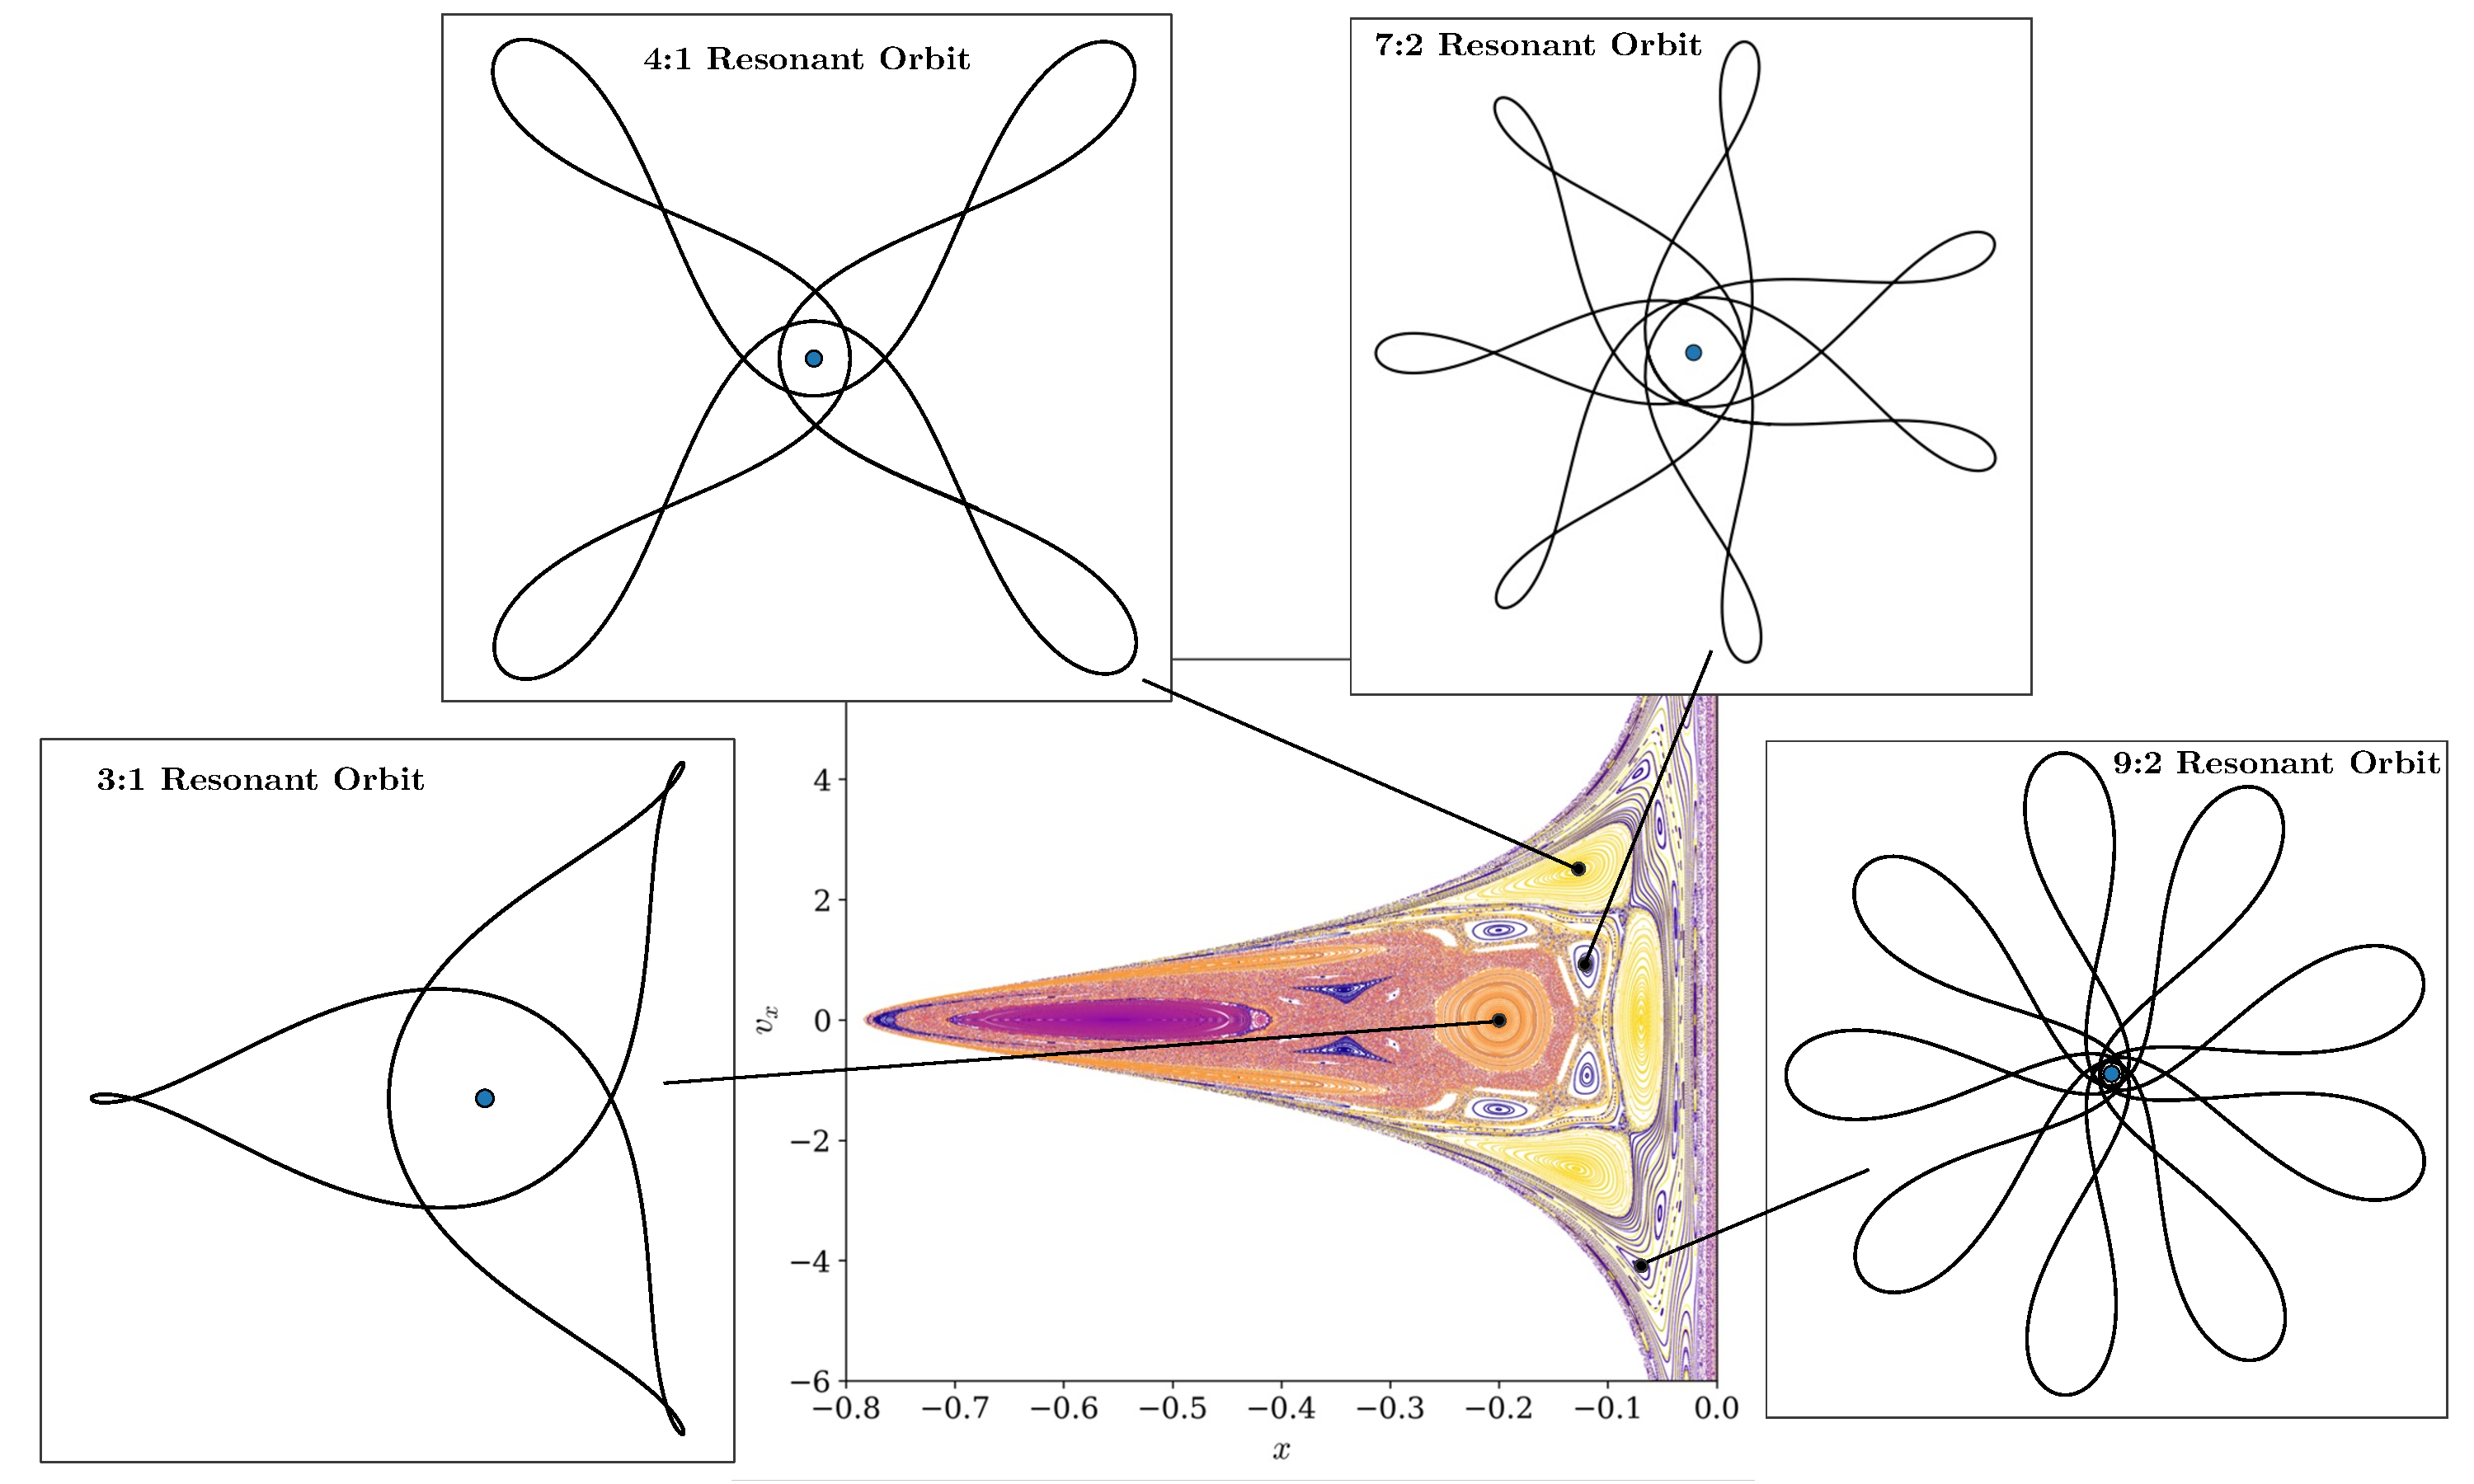
\includegraphics[width=1.0\linewidth]{images/Chaotic_sea_figure.pdf}
    \caption{Resonant orbits corresponding to islands of fixed-energy Poincaré map at $C=3.2$.}
    \label{fig:C_3.2_with_orbits}
\end{figure}
\newpage
